\documentclass[aspectratio=169,11pt]{beamer}
% ==========================================================================
%  KSA lecture-slide theme  =  stock beamer "Boadilla"  +  KSA colour theme
%  brand colours sampled from the official KSA symbol mark:
%    Deep Prussian Blue  #2E3192   (지성 - intellect)
%    Golden Gray         #D6CBB1   (감성 - sensibility)
%  Engine: XeLaTeX.  Usage:
%    \documentclass[aspectratio=169,11pt]{beamer}
%    \input{../../theme/ksa-theme.tex}
%  Each deck lives in its own slides/kor/<deck>/ folder together with its
%  own images; ../../figs/ is kept only as a fallback for the shared cache.
% ==========================================================================

\usepackage{fontspec}
\usepackage{amsmath,amssymb}
\usepackage{graphicx}
\graphicspath{{figs/}{./}{../../../figs/}}
\usepackage{booktabs}
\usepackage{listings}
\usepackage{varwidth}

% ---- fonts (no ctex/xeCJK on this box -> fontspec drives CJK directly) -----
\defaultfontfeatures{Ligatures=TeX}
\setmainfont{Noto Sans CJK KR}
\setsansfont{Noto Sans CJK KR}
\setmonofont{Noto Sans Mono CJK KR}[Scale=0.92]

% ---- base theme: stock Boadilla ------------------------------------------
\usetheme{Boadilla}
\usefonttheme{professionalfonts}
\setbeamertemplate{navigation symbols}{}

% ---- KSA colour theme (recolour the stock theme) --------------------------
\definecolor{ksablue}{HTML}{2E3192}
\definecolor{ksabluedk}{HTML}{20226A}
\definecolor{ksagold}{HTML}{D6CBB1}
\definecolor{ksagolddk}{HTML}{A9976B}
\definecolor{ksared}{HTML}{C0392B}
\definecolor{ksagray}{HTML}{5B5B5B}

\setbeamercolor{structure}{fg=ksablue}
\setbeamercolor{alerted text}{fg=ksared}

\setbeamercolor{palette primary}{fg=white,           bg=ksablue}
\setbeamercolor{palette secondary}{fg=white,         bg=ksablue!85!black}
\setbeamercolor{palette tertiary}{fg=white,          bg=ksabluedk}
\setbeamercolor{titlelike}{fg=ksablue}
\setbeamercolor{frametitle}{fg=ksablue,bg=}
\setbeamercolor{title}{fg=ksablue}
\setbeamercolor{author}{fg=ksagray}
\setbeamercolor{institute}{fg=ksagray}
\setbeamercolor{block title}{fg=white,bg=ksablue}
\setbeamercolor{block body}{fg=black!85,bg=ksablue!6}
\setbeamercolor{item}{fg=ksablue}
\setbeamercolor{section in toc}{fg=black!85}

\setbeamerfont{frametitle}{series=\bfseries}
\setbeamerfont{title}{series=\bfseries}

% ---- footline:  KSA mark | "Made by ..." | n / N   (matches reference) ----
\newcommand{\ksacredit}{}
\setbeamertemplate{footline}{%
  \hbox{%
    \begin{beamercolorbox}[wd=.18\paperwidth,ht=2.6ex,dp=1.5ex,leftskip=1.1em]{}%
      \raisebox{-0.35ex}{\includegraphics[height=2.0ex]{ksa-logo.png}}%
    \end{beamercolorbox}%
    \begin{beamercolorbox}[wd=.64\paperwidth,ht=2.6ex,dp=1.5ex,center]{}%
      {\scriptsize\color{ksagray}\ksacredit}%
    \end{beamercolorbox}%
    \begin{beamercolorbox}[wd=.18\paperwidth,ht=2.6ex,dp=1.5ex,rightskip=1.1em]{}%
      \hfill{\scriptsize\color{ksablue}\insertframenumber\,/\,\inserttotalframenumber}%
    \end{beamercolorbox}%
  }%
  \vskip2pt
}

% ---- section divider: stock \sectionpage, KSA-coloured -------------------
\setbeamertemplate{section page}{%
  \begingroup\centering
    {\color{ksagolddk}\rule{0.16\paperwidth}{1pt}}\par\vskip1.0em
    {\usebeamerfont{title}\color{ksablue}\insertsectionhead\par}\vskip1.0em
    {\color{ksagolddk}\rule{0.16\paperwidth}{1pt}}\par
  \endgroup
}
\AtBeginSection[]{\begin{frame}[plain,noframenumbering]\vfill\sectionpage\vfill\end{frame}}

% ---- code listings ------------------------------------------------------------
\lstdefinestyle{ksa}{%
  basicstyle=\ttfamily\scriptsize,
  keywordstyle=\color{ksablue}\bfseries,
  commentstyle=\color{ksagray}\itshape,
  stringstyle=\color{ksagolddk},
  numberstyle=\tiny\color{ksagray},
  backgroundcolor=\color{ksablue!6},
  frame=leftline, framerule=1.4pt, rulecolor=\color{ksablue},
  xleftmargin=1em, aboveskip=0.8em, belowskip=0.4em,
  showstringspaces=false, breaklines=true, language=Python,
}
\lstset{style=ksa}

% ---- handy macros -----------------------------------------------------------
\newcommand{\kb}[1]{\textbf{\color{ksablue}#1}}   % blue keyword
\newcommand{\kq}[1]{\textbf{\color{ksared}#1}}    % red key-question

\setbeamerfont{title}{series=\bfseries,size=\fontsize{24}{30}\selectfont}
\setbeamerfont{subtitle}{series=\bfseries,size=\fontsize{14}{18}\selectfont}
\setbeamerfont{author}{size=\normalsize}
\setbeamerfont{institute}{size=\small}
\graphicspath{{figs/}{../../../../assets/}}
\makeatletter
\newcommand{\markpage}[1]{\protected@write\@auxout{}{\string\newlabel{#1}{{\the\c@framenumber}{}}}\hypertarget{#1}{}}
\newcommand{\pref}[1]{\hyperlink{#1}{\textcolor{ksagolddk}{(p.\ref{#1})}}}
\makeatother

\renewcommand{\ksacredit}{Machine Learning 1 \,\textperiodcentered\, PCA}
\title{PCA 주성분 분석 (Principal Component Analysis)}
\subtitle{가장 넓게 퍼진 방향으로 그림자를 낸다}
\author{Machine Learning 1}
\institute{한국과학영재학교 (KSA)}
\date{}
\begin{document}
\begin{frame}[plain,noframenumbering]\titlepage\end{frame}


% --- 오늘의 질문
\begin{frame}{오늘의 질문: 숫자 두 개를 하나로 줄이려면?}
\vfill
\begin{columns}[c]
\column{0.42\linewidth}\centering
\renewcommand{\arraystretch}{1.1}
{\normalsize\begin{tabular}{ccc}
학생 & 수학 & 물리\\\hline
1 & 95 & 92\\
2 & 35 & 47\\
3 & 73 & 76\\
$\vdots$ & $\vdots$ & $\vdots$\\
20 & 65 & 56
\end{tabular}}\\[0.4em]
{\small 20명 점수 (설명용 예시)}
\column{0.56\linewidth}
{\large 학생마다 숫자 2개 $\to$ \kb{1개}로 줄이고 싶다}\\[0.6em]
{\large 수학 점수만 남기면?}\\[0.2em]
{\large 평균을 내면?}\\[0.2em]
{\large 가장 \textbf{정보를 많이 남기는} 한 숫자는?}\\[0.8em]
{\small 특징이 수십 · 수백 개면: 그림으로 보고, 저장을 줄이고, 다음 모델을 빠르게}
\end{columns}
\vfill
\note{학생 20명의 수학과 물리 점수가 있습니다. 설명을 위해 만든 예시입니다. 학생마다 숫자가 두 개인데, 이걸 하나로 줄이고 싶습니다. 수학 점수만 남길 수도 있고, 두 점수의 평균을 낼 수도 있죠. 어떤 한 숫자가 정보를 가장 많이 남길까요? 특징이 수십, 수백 개일 때 이렇게 줄이면 그림으로 볼 수 있고, 저장 공간도 줄고, 다음 모델도 빨라집니다. 오늘은 이걸 하는 가장 기본적인 방법, 주성분 분석 PCA를 배웁니다.}
\end{frame}

% --- 그림자
\begin{frame}{그림자를 내 보자}
\markpage{shadow}
\vfill
\centering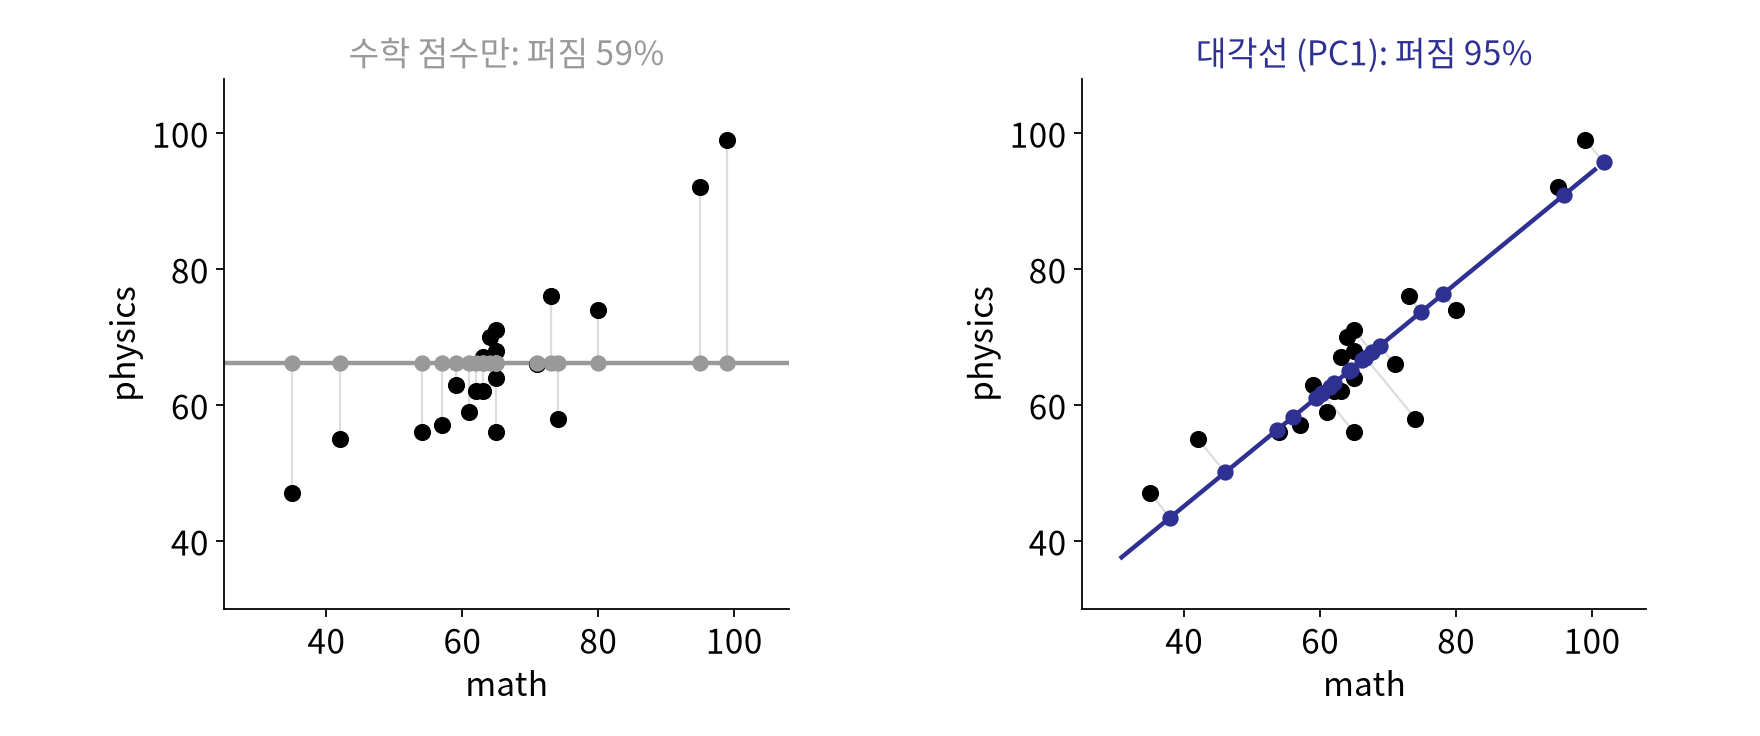
\includegraphics[width=0.8\linewidth]{pc_shadow.png}\par\vskip0.2em
{\large 점을 한 직선에 수직으로 내리면 (그림자 = 투영) 숫자 하나가 된다}\\[0.2em]
{\large 그림자가 \kb{넓게 퍼질수록} 학생들의 차이가 많이 남는다 \quad 수학 축 59\% \quad 대각선 95\%}
\vfill
\note{점들을 한 직선에 수직으로 내리면, 직선 위의 위치, 즉 숫자 하나가 됩니다. 이걸 그림자 또는 투영이라고 합니다. 왼쪽은 수학 축에 그림자를 낸 것, 그러니까 수학 점수만 남긴 겁니다. 그림자가 퍼진 정도, 분산이 원래 퍼짐의 59퍼센트입니다. 오른쪽은 대각선 방향에 그림자를 낸 것인데, 95퍼센트가 남습니다. 그림자가 넓게 퍼질수록 학생들 사이의 차이가 많이 남은 겁니다. 반대로 그림자가 한 점에 몰리면 모두 같은 숫자가 되어 정보가 없어지죠.}
\end{frame}

% --- 각도
\begin{frame}{방향을 돌려 보면}
\vfill
\centering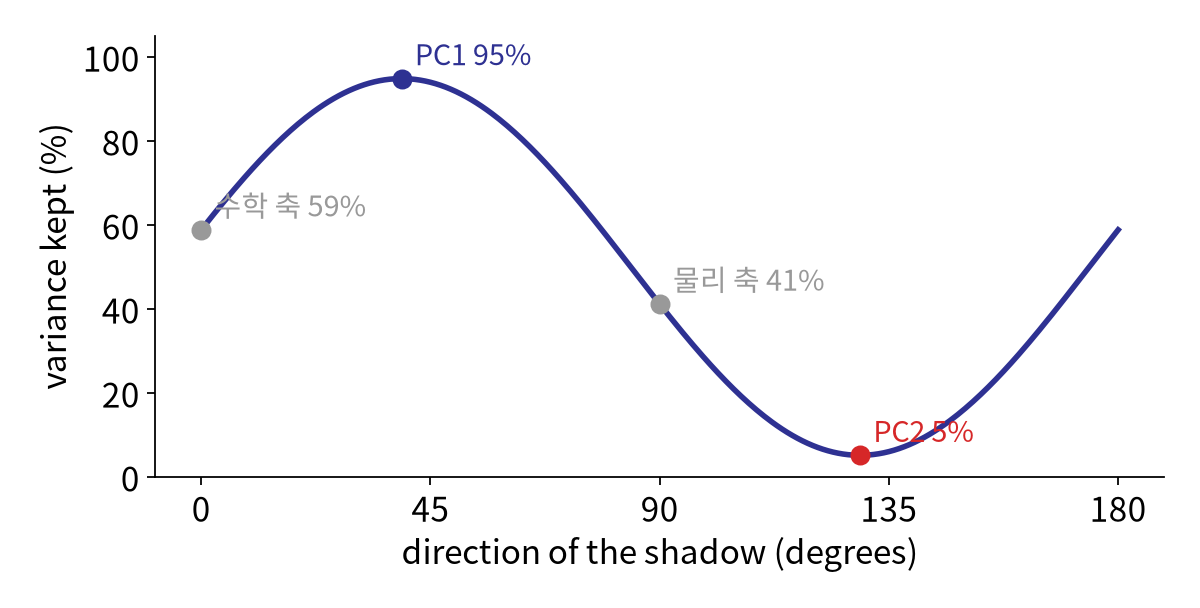
\includegraphics[width=0.66\linewidth]{pc_angle.png}\par\vskip0.2em
{\large 가장 넓게 퍼지는 방향 (39°) = \textcolor{ksablue}{\textbf{제1 주성분 PC1}} \quad 남는 퍼짐 \kb{95\%}}\\[0.2em]
{\large 그와 수직 (129°) = \textcolor{ksared}{\textbf{PC2}} \quad 나머지 \kq{5\%} \quad 두 비율의 합 = 100\%}
\vfill
\note{그림자를 내는 방향을 0도부터 180도까지 돌려 보면, 남는 퍼짐이 이렇게 물결칩니다. 0도, 수학 축은 59퍼센트, 90도, 물리 축은 41퍼센트입니다. 39도 근처에서 가장 넓어 95퍼센트가 남습니다. 이 방향이 제1 주성분, PC1입니다. 그와 수직인 129도에서 가장 좁아 5퍼센트인데, 이게 제2 주성분 PC2입니다. 서로 수직인 두 방향의 퍼짐을 더하면 항상 100퍼센트입니다.}
\end{frame}

% --- PC 의 뜻
\begin{frame}{주성분의 뜻}
\vfill
\begin{columns}[c]
\column{0.4\linewidth}\centering
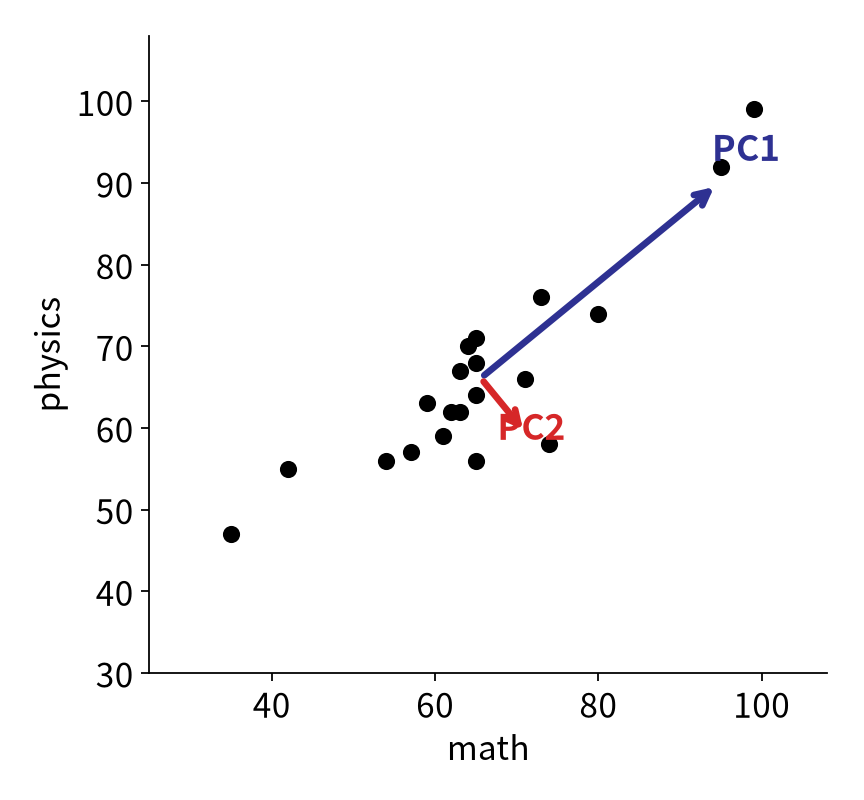
\includegraphics[width=\linewidth]{pc_axes.png}
\column{0.58\linewidth}
\renewcommand{\arraystretch}{1.5}
{\large\begin{tabular}{lll}
\textcolor{ksablue}{PC1} & $0.77 \cdot$ 수학 $+ 0.63 \cdot$ 물리 & ``둘 다 잘함''\\
\textcolor{ksared}{PC2} & $0.63 \cdot$ 수학 $- 0.77 \cdot$ 물리 & ``수학이 더 셈''
\end{tabular}}\\[0.6em]
{\large 주성분 = 원래 특징들의 \textbf{가중합} (방향 벡터, 길이 1)}\\[0.3em]
{\large 두 점수가 함께 움직여 (상관) 한 방향에 몰린다}\\[0.6em]
{\small 평균을 뺀 점수에 곱한다 (평균: 수학 65.6, 물리 66.1)}
\end{columns}
\vfill
\note{주성분은 원래 특징들의 가중합입니다. PC1은 0.77 곱하기 수학 더하기 0.63 곱하기 물리, 둘 다 높을수록 커지니 전체적으로 잘한다는 뜻입니다. PC2는 0.63 곱하기 수학 빼기 0.77 곱하기 물리, 수학이 물리보다 셀수록 커집니다. 이 방향 벡터들은 길이가 1입니다. 수학과 물리 점수가 함께 움직이니까, 즉 상관이 크니까, 퍼짐이 대부분 한 방향에 몰린 겁니다. 실제로는 평균, 수학 65.6과 물리 66.1을 먼저 뺀 점수에 곱합니다.}
\end{frame}

% --- 식
\begin{frame}{식으로: 공분산 행렬의 고유벡터}
\markpage{formula}
\vfill
\centering
{\large 방향 $\mathbf{u}$ ($\|\mathbf{u}\| = 1$) 로 그림자를 냈을 때의 분산 \quad $= \mathbf{u}^\top S\, \mathbf{u}$, \quad $S$ = 공분산 행렬}\vskip0.4em
{\LARGE\[ \max_{\|\mathbf{u}\| = 1} \mathbf{u}^\top S \mathbf{u} \quad \Rightarrow \quad S \mathbf{u} = \lambda \mathbf{u} \]}\vskip0.2em
{\large 답 = $S$ 의 \textbf{고유벡터}, \quad 그 방향의 분산 = \textbf{고유값} $\lambda$}\\[0.6em]
\renewcommand{\arraystretch}{1.3}
{\large\begin{tabular}{ll}
$S = \begin{pmatrix} 217.8 & 162.8 \\ 162.8 & 152.4 \end{pmatrix}$ &
$\lambda^2 - 370.2\,\lambda + 6685.7 = 0$ \quad $\Rightarrow$ \quad $\lambda_1 = \kb{351.2}, \ \lambda_2 = 19.0$
\end{tabular}}\\[0.4em]
{\large 설명 분산 비율 \quad $351.2 / 370.2 = \kb{95\%}$}
\vfill
\note{식으로 쓰면, 길이 1인 방향 u로 그림자를 냈을 때의 분산은 u 전치 S u입니다. S는 공분산 행렬입니다. 이걸 최대로 하는 u를 찾으면, 라그랑주 승수법으로 S u는 람다 u라는 식이 나옵니다. 즉 답은 S의 고유벡터이고, 그 방향의 분산이 고유값 람다입니다. 우리 예에서 S는 수학 분산 217.8, 물리 분산 152.4, 공분산 162.8입니다. 2 곱하기 2 행렬의 고유값은 람다 제곱 빼기 대각합 370.2 람다 더하기 행렬식 6685.7이 0인 식에서 나오고, 351.2와 19.0입니다. 351.2 나누기 370.2, 95퍼센트가 설명 분산 비율입니다.}
\end{frame}

% --- 절차
\begin{frame}{PCA 절차}
\vfill
\centering
\renewcommand{\arraystretch}{1.6}
{\large\begin{tabular}{rl}
1 & 특징마다 \textbf{평균을 뺀다} (단위가 다르면 표준화까지)\\
2 & 공분산 행렬 $S$ 를 구한다 ($d \times d$)\\
3 & 고유값 · 고유벡터를 구해 큰 순서로 정렬\\
4 & 위에서 $k$ 개 방향에 그림자 $\to$ 숫자 $k$ 개 \quad (설명 분산 비율로 $k$ 를 고른다)
\end{tabular}}\vskip0.8em
{\large 붓꽃 4개 측정값: 그대로 92.5 + 5.3 = \kb{97.8\%} \quad 표준화하면 73.0 + 22.9 = 95.9\%}\\[0.2em]
{\small 꽃잎 길이처럼 cm 값이 큰 특징이 분산을 독차지 $\to$ 단위가 다르면 표준화가 필요}
\vfill
\note{PCA의 절차를 정리하면 넷입니다. 첫째, 특징마다 평균을 빼서 중심을 맞춥니다. 단위가 다르면 표준편차로 나눠 표준화까지 합니다. 둘째, 공분산 행렬을 구합니다. 셋째, 고유값과 고유벡터를 구해 큰 순서로 정렬합니다. 넷째, 위에서 k개 방향에 그림자를 내 숫자 k개로 줄입니다. k는 설명 분산 비율을 보고 고릅니다. 붓꽃의 측정값 4개를 그대로 PCA하면 2개로 97.8퍼센트가 남고, 표준화하면 95.9퍼센트입니다. 표준화 전에는 꽃잎 길이처럼 값의 범위가 큰 특징이 분산을 독차지하기 때문입니다.}
\end{frame}

% --- 붓꽃 / 숫자
\begin{frame}{4차원 붓꽃을 평면에}
\vfill
\begin{columns}[c]
\column{0.5\linewidth}\centering
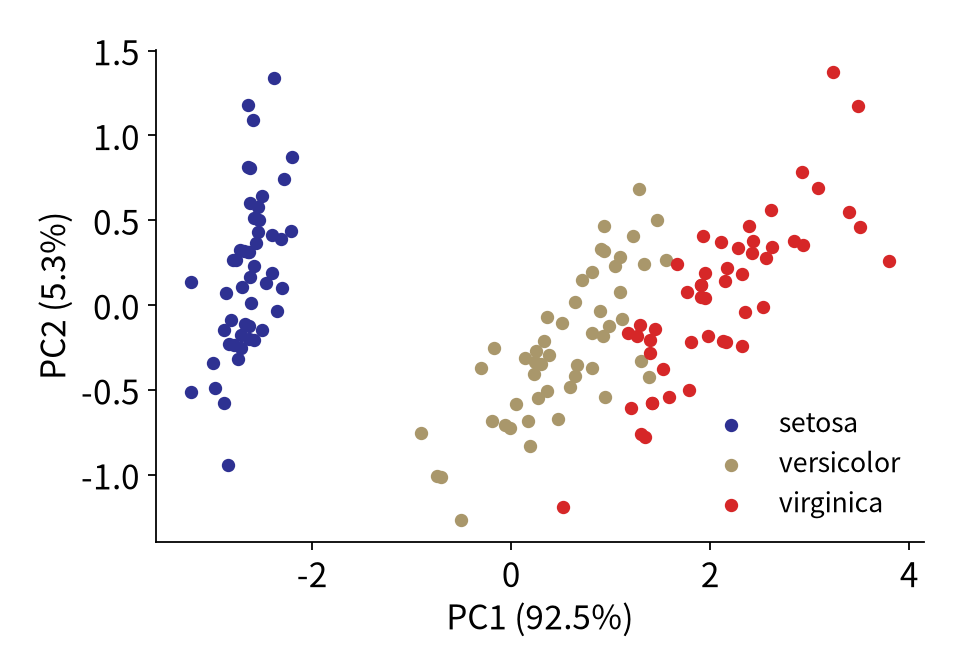
\includegraphics[width=\linewidth]{pc_iris.png}
\column{0.48\linewidth}
{\large 붓꽃 150송이, 측정값 4개}\\{\small (꽃받침 · 꽃잎의 길이 · 너비)}\\[0.6em]
{\large PC1 하나로 setosa 가 \textbf{깨끗이} 갈라진다}\\[0.6em]
{\large 이름표를 쓰지 않았다: \kb{비지도 학습}}\\[0.2em]
{\small 색은 그린 뒤에 칠했다}
\end{columns}
\vfill
\note{붓꽃 150송이의 측정값 4개를 PC1, PC2 두 숫자로 줄여 평면에 그렸습니다. PC1 하나만으로 setosa가 깨끗하게 갈라지고, 나머지 두 종도 꽤 나뉩니다. 중요한 점은 PCA가 품종 이름표를 전혀 쓰지 않았다는 겁니다. 측정값만 보고 퍼짐이 큰 방향을 찾았을 뿐입니다. 이런 걸 비지도 학습이라 합니다. 색은 그린 뒤에 칠한 겁니다.}
\end{frame}

% --- 압축
\begin{frame}{압축: 손글씨 숫자 64칸을 몇 개로?}
\markpage{digit}
\vfill
\centering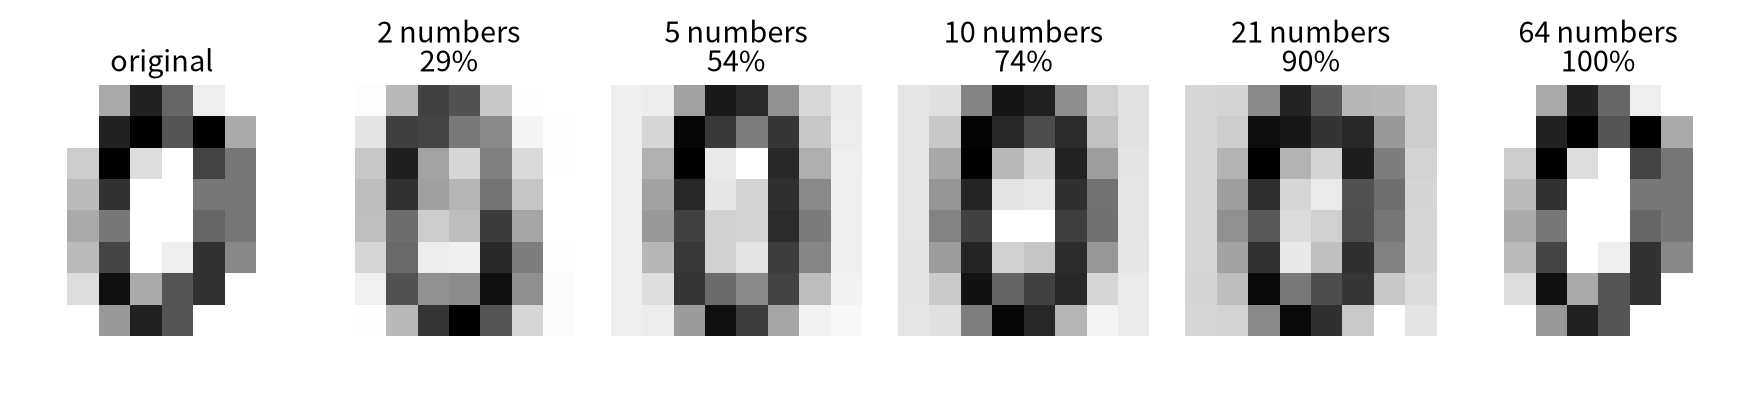
\includegraphics[width=0.82\linewidth]{pc_digit.png}\par
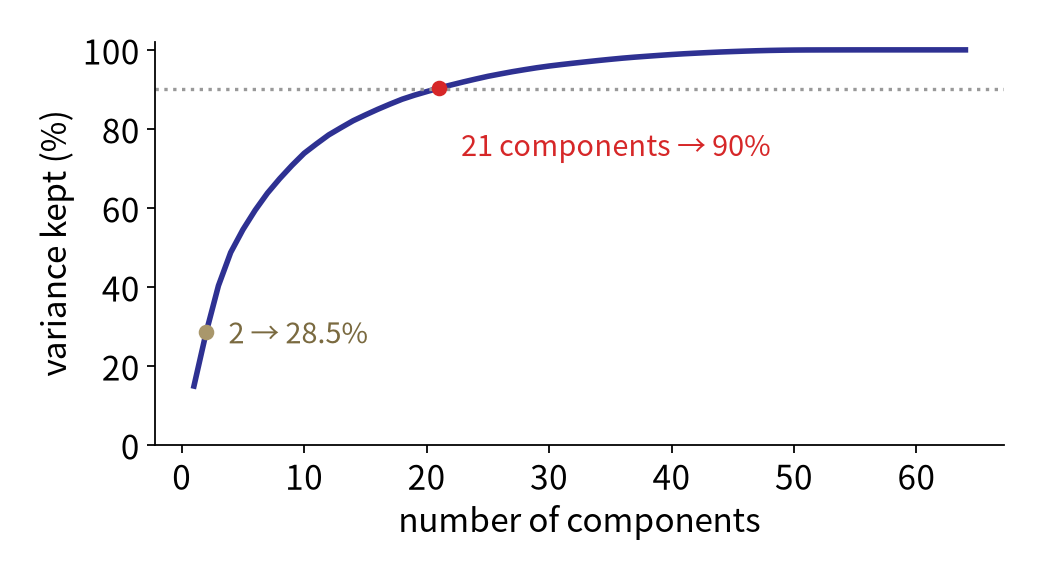
\includegraphics[width=0.46\linewidth]{pc_digit_curve.png}\par
{\large 1,797장, 8 × 8 = 64칸 \quad 성분 \kb{21개}로 90\% \quad 2개로는 28.5\% 뿐}
\vfill
\note{손글씨 숫자 이미지 1797장은 한 장이 8 곱하기 8, 숫자 64개입니다. PCA로 성분 k개만 남겼다가 다시 64칸으로 되돌려 보면, 2개로는 흐릿하지만 0의 모양은 보이고, 21개면 퍼짐의 90퍼센트가 남아 거의 원래 모습입니다. 64칸을 21개로 3분의 1로 줄인 셈입니다. 반대로 2개로는 28.5퍼센트밖에 안 남습니다. 그래서 숫자 1797장을 PCA 두 축으로 평면에 그리면 숫자끼리 뒤엉킵니다. 다음 시간 t-SNE가 이 문제를 다룹니다.}
\end{frame}

% --- 쓰임과 한계
\begin{frame}{쓰임과 한계}
\vfill
\centering
\renewcommand{\arraystretch}{1.5}
{\large\begin{tabular}{ll}
고유얼굴 (1991) & Turk \& Pentland: 얼굴 사진의 주성분으로 얼굴 인식\\
시각화 & 수십 차원 데이터를 2 · 3차원으로 먼저 그려 본다\\
전처리 & 특징을 줄여 다음 모델을 빠르게, 잡음 줄이기\\
유전체 & 사람들의 유전 변이 PC1 · PC2 가 지도처럼 출신 지역을 드러낸다
\end{tabular}}\vskip0.8em
{\large 한계: \textbf{직선} 방향의 그림자만 \quad 휘어진 구조, 뭉친 무리는 놓친다 $\to$ t-SNE}
\vfill
\note{PCA는 쓰임이 넓습니다. 1991년 터크와 펜틀랜드는 얼굴 사진들의 주성분, 고유얼굴로 얼굴을 인식했습니다. 수십 차원 데이터를 2, 3차원으로 먼저 그려 보는 데에도, 특징을 줄여 다음 모델을 빠르게 하거나 잡음을 줄이는 데에도 씁니다. 유럽 사람들의 유전 변이에 PCA를 하면 PC1, PC2 평면이 유럽 지도처럼 출신 지역을 드러낸다는 유명한 연구도 있습니다. 한계는 직선 방향의 그림자만 본다는 겁니다. 휘어진 구조나 여러 무리로 뭉친 데이터는 놓칩니다. 이걸 보완하는 게 다음 시간 t-SNE입니다.}
\end{frame}

% --- 문제풀이
\begin{frame}{문제풀이}
\vfill
\begin{enumerate}
\item 고유값이 6, 3, 1 인 3차원 데이터를 2차원으로 줄이면 퍼짐이 몇 \% 남나?\vskip0.8em
\item $S = \begin{pmatrix} 5 & 0 \\ 0 & 1 \end{pmatrix}$ 이면 PC1 방향과 설명 분산 비율은?\vskip0.8em
\item PC1 이 $(0.77, 0.63)$ 일 때, 평균을 뺀 점수 (10, 10) 인 학생의 PC1 값은?\vskip0.8em
\item 키 (cm) 와 몸무게 (kg) 를 표준화 없이 PCA 하면 무엇이 문제일까? 키를 mm 로 바꾸면?
\end{enumerate}
\vfill
\note{1번 답. 6 더하기 3을 10으로 나눠 90퍼센트입니다. 2번 답. 이미 대각 행렬이니 PC1은 첫 번째 축 방향 1, 0이고, 5 나누기 6, 약 83퍼센트입니다. 3번 답. 0.77 곱하기 10 더하기 0.63 곱하기 10, 14입니다. 4번 답. 단위에 따라 분산이 달라지니, 숫자가 큰 특징이 PC1을 차지합니다. 키를 mm로 바꾸면 분산이 100배가 되어 PC1이 거의 키 방향이 됩니다. 그래서 단위가 다르면 표준화합니다.}
\end{frame}

% --- 실습
\begin{frame}{실습}
\vfill
\centering\begin{tabular}{rl}
\large 1 & 학생 점수: 각도별 퍼짐 $\to$ 공분산 · 고유분해로 PC1 (95\%) 직접 구하기\\[0.5em]
\large 2 & \texttt{sklearn PCA} 와 비교, 붓꽃 4 $\to$ 2차원 (표준화 전후)\\[0.5em]
\large 3 & 손글씨 숫자 압축 · 복원: 성분 수 바꾸기
\end{tabular}\vskip1em
\href{https://colab.research.google.com/github/SuminHan/book-ml/blob/main/slides/v2/ml1/week14/pca/lab/pca.ipynb}{\textcolor{ksagolddk}{▶ Colab에서 실습 노트북 열기}}
\vfill
\note{실습은 세 부분입니다. 첫째, 학생 점수로 각도별 퍼짐을 재고, 공분산 행렬의 고유분해로 PC1을 직접 구합니다. 둘째, sklearn PCA와 비교하고 붓꽃을 표준화 전후로 2차원으로 줄여 봅니다. 셋째, 손글씨 숫자를 성분 수를 바꿔 가며 압축하고 복원합니다.}
\end{frame}

% --- 정리
\begin{frame}{정리}
\vfill
\centering\large\begin{tabular}{l}
\textbf{PCA}: 그림자가 \kb{가장 넓게 퍼지는} 방향 = PC1, 그와 수직으로 PC2, $\cdots$\\[0.5em]
= 공분산 행렬의 고유벡터, 퍼짐 = 고유값 \quad 학생 점수: 수학만 59\% $\to$ PC1 95\%\\[0.5em]
평균 빼기 (단위 다르면 표준화) $\to$ $S$ $\to$ 고유분해 $\to$ 위 $k$ 개로 투영\\[0.5em]
붓꽃 4 $\to$ 2: 97.8\% \quad 숫자 64 $\to$ 21: 90\% \quad 한계: 직선만 $\to$ t-SNE
\end{tabular}
\vfill
\note{정리합니다. PCA는 그림자가 가장 넓게 퍼지는 방향을 PC1으로, 그와 수직인 방향 중 가장 넓은 방향을 PC2로 찾습니다. 이 방향들은 공분산 행렬의 고유벡터이고, 퍼짐은 고유값입니다. 학생 점수에서 수학만 남기면 59퍼센트, PC1은 95퍼센트였습니다. 절차는 평균 빼기, 공분산, 고유분해, 투영입니다. 붓꽃은 4개에서 2개로 97.8퍼센트, 숫자는 64칸에서 21개로 90퍼센트가 남았습니다. 직선만 본다는 한계는 다음 시간 t-SNE로 이어집니다.}
\end{frame}
\end{document}
